\documentclass[../main.tex]{subfiles}

\begin{document}
\section{Theory}
\subsection{Logistic regression}
Logistic regression is a method for classifying a set of input variables \ensuremath{\boldsymbol{x}} to an output or class \ensuremath{y_i, i=1,2, \ldots,K} where $K$ is the number of classes. The review in this section is based on Hastie et al. \cite[ch.~4]{HastieTrevor2009EoSL},  and the reader is referred to this book for a more detailed explanation of topic. The prediction of output classes which the input variables belongs to is based on the design matrix \ensuremath{\boldsymbol{X}\in\mathbb{R}^{n\times p}} that contains $n$ samples that each carry $p$ features. We distinct between \textit{hard} and \textit{soft classification}, which determines the input variable to a class deterministically or the probability that a given variable belongs in a certain class. The logistic regression model is given on the form
 
\begin{align}
    \begin{split}
        \log\frac{p(G=1|X=x)}{p(C=K|X=x)}&=\beta_{10}+\beta_1^Tx \\
        \log\frac{p(G=2|X=x)}{p(C=K|X=x)}&=\beta_{20}+\beta_2^Tx \\
        &\vdots\\ 
        \log\frac{p(G=K-1|X=x)}{p(C=K|X=x)}&=\beta_{(K-1)0}+\beta_{K-1}^Tx.
    \end{split}
\end{align}

We consider the binary, two-class case with \ensuremath{y_i \in [0,1]}. The probability that a given input variable $x_i$ belongs in class $y_i$ is given by the Sigmoid-function (also called logistic function):
\begin{align}
    p(x) = \frac{e^x}{1+e^x}=\frac{1}{1+e^{-x}}.
    \label{eq:sigmoid}
\end{align}

A set of predictors, \ensuremath{\boldsymbol{\beta}}, which we want to estimate with our data then gives the probabilities 

\begin{align}
    p(y_i=1|x_i,\boldsymbol{\beta})=\frac{\exp\left(\boldsymbol{\beta}^Tx_i\right)}{1+\exp\left(\boldsymbol{\beta}^Tx_i\right)} \\
    p(y_i=0|x_i,\boldsymbol{\beta})=1-p(y_i=1|x_i,\boldsymbol{\beta}).
\end{align} We define the set of all possible outputs in our data set \ensuremath{\mathcal{D}(x_i,y_i)}. Further, we assume that all samples \ensuremath{\mathcal{D}(x_i,y_i)} are independent and identically distributed. Now we can approximate the total likelihood for all possible outputs of \ensuremath{\mathcal{D}} by the product of the individual probabilities \cite[p.~120]{HastieTrevor2009EoSL} of a specific output $y_i$:

\begin{align}
    P(\mathcal{D}|\boldsymbol{\beta}) = \prod_{i=1}^n[p(y_i=1|x_i\boldsymbol{\beta})]^{y_i}[1-p(y_i=1|x_i,\boldsymbol{\beta})]^{1-y_i}.
    \label{eq:likelihood}
\end{align} We want to maximize this probability by using the maximum likelihood estimator (MLE). By taking the logarithm of \cref{eq:likelihood}, we obtain the log-likelihood in \ensuremath{\boldsymbol{\beta}}

\begin{align}
    \log P(\mathcal{D}|\boldsymbol{\beta}) = \sum_{i=1}^n[y_i\log p(y_i=1|x_i\boldsymbol{\beta})+(1-y_i)\log(1-p(y_i=1|x_i,\boldsymbol{\beta}))].
    \label{eq:log-likelihood}
\end{align}

By reordering the logarithms and taking the negative of \cref{eq:log-likelihood}, we obtain the \textit{cross entropy}

\begin{align}
    \mathcal{C}(\boldsymbol{\beta})=-\sum_{i=1}^n\left[y_i\boldsymbol{\beta}^Tx_i-\log\left(1+\exp\left(\boldsymbol{\beta}^Tx_i\right)\right)\right].
    \label{eq:cross-entropy}
\end{align} The cross entropy is used as our cost function for logistic regression. We minimize the cross entropy, which is the same as maximizing the log-likelihood, and obtain

\begin{align}
    \frac{\partial\mathcal{C}(\boldsymbol{\beta})}{\partial\boldsymbol{\beta}}=-\sum_{i=1}^nx_i(y_i-p(y_i=1|x_i,\boldsymbol{\beta}))=0.
\end{align} The second derivative of this quantity is

\begin{align}
    \frac{\partial^2\mathcal{C}(\boldsymbol{\beta})}{\partial\boldsymbol{\beta}\partial\boldsymbol{\beta}^T}=\sum_{i=1}^nx_ix_i^Tp(y_i=1|x_i,\boldsymbol{\beta})(1-p(y_i=1|x_i,\boldsymbol{\beta})).
\end{align} These expressions can be written more compactly by defining the diagonal matrix \ensuremath{\boldsymbol{W}} with elements \ensuremath{p(y_i=1|x_i,\boldsymbol{\beta})(1-p(y_i=1|x_i,\boldsymbol{\beta}))}, \ensuremath{\boldsymbol{y}} as the vector with our $y_i$s values and \ensuremath{\boldsymbol{p}} as the vector of fitted probabilities. We can then express the first and second derivatives in matrix form

\begin{align}
    \frac{\partial\mathcal{C}(\boldsymbol{\beta})}{\partial\boldsymbol{\beta}}&=-\boldsymbol{X}^T(\boldsymbol{y}-\boldsymbol{p}) \\
    \frac{\partial^2\mathcal{C}(\boldsymbol{\beta})}{\partial\boldsymbol{\beta}\partial\boldsymbol{\beta}^T} &= \boldsymbol{X}^T\boldsymbol{W}\boldsymbol{X},
\end{align} also known as the Jacobian and Hessian matrices, respectively. We will use the stochastic gradient descent (SGD) (\cref{sec:sgd}) to find the optimal parameter \ensuremath{\boldsymbol{\beta}}. 


\subsection{Stochastic Gradient Descent}\label{sec:sgd}
\textit{Gradient descent} describes the process of finding a local minimum of a function (the cost function, in our case) by following the negative value of the gradient at each point, stepwise. \textit{Stochastic gradient descent} or SDG is a way of increasing the numerical efficiency of this process, by doing this process stochastically.

This involves randomly dividing the training data into a given number of \textit{mini batches}. For each mini batch, the gradient is found by averaging the gradient value each mini batch sample has. Then the weights and biases are updated (take a step down the "slope") and the process is repeated for the rest of the mini batches. The updating done at each mini batch is expressed mathematically as

\begin{align*}
    w&\rightarrow w' = w - \frac{\eta}{m}\sum_i^m \nabla C_{i,w} \\
    b&\rightarrow b' = b - \frac{\eta}{m}\sum_i^m \nabla C_{i,b},
\end{align*}

where $m$ is the number of data points in the mini batches and $\nabla C_i$ is the gradient of the cost function at each individual data point. After exhausting all the training data, we have finished a so-called \textit{epoch}, of which we can perform as many as necessary.

\subsection{Neural networks}
Neural networks is a machine learning technique vaguely inspired by our understanding of how networks of neurons function in the brain. There are several types of neural networks. In this work, we study a multi-layer perception (MLP). The MLP is characterized by one or more \textit{hidden layers} between the input and output layers. Each hidden layer consists of several \textit{neurons} (also called \textit{nodes}). The neurons in each layer is not connected to each other, but 
all nodes of a layer is connected to every neuron in the previous layer. We say that we have a \textit{fully connected layer}. 
\Cref{fig:simple_network} shows an example of a neural network used for binary classification, while \cref{fig:multi_class_network} display an  example of a neural network used for a multi-class classification problem. In both sub-figures of \cref{fig:network_diagrams}, we see that the inputs are fed through the network and processed, resulting in an output. 

\begin{figure}
     \centering
     \begin{subfigure}[b]{0.35\textwidth}
         \centering
         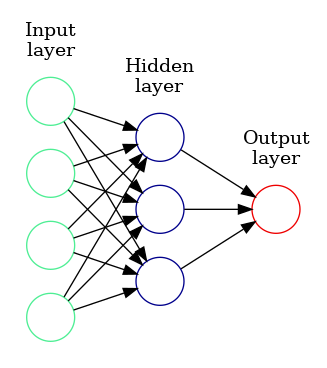
\includegraphics[width=\textwidth]{doc/assets/simple_neural_network_diagram.png}
         \caption{}
         \label{fig:simple_network}
     \end{subfigure}
     \quad
     \begin{subfigure}[b]{0.6\textwidth}
         \centering
         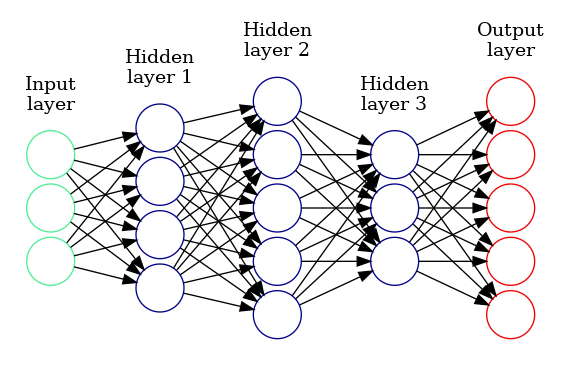
\includegraphics[width=\textwidth]{doc/assets/multi_class_neural_network_diagram.png}
         \caption{}
         \label{fig:multi_class_network}
     \end{subfigure}
        \caption{Schematic diagram of a neural network with: (a) four inputs, one hidden layer of three neurons and one output layer with one neuron. (b) three inputs, three hidden layers (four, five and three neurons) and one output layer with five neurons. Note that we have only fully connected layers.}
        \label{fig:network_diagrams}
\end{figure}

\subsubsection{Forward feeding}
As we can see in both example network diagrams in \cref{fig:network_diagrams}, each neuron has one or multiple inputs. In the following, we consider the $j^{\text{th}}$ neuron in the $l^{\text{th}}$ layer. Each of the inputs is multiplied by a weight, $w_j$, when passed into a neuron, and the result is called $z_j$. An activation function \ensuremath{a(z_j)=a_j} evaluates the signal, $a_j$ becomes the output from each neuron. We denote the weight associated with the input from the $k^{\text{th}}$ neuron in the previous layer $w_{jk}^l$. Further, wee add a bias, $b_j$ to each of the neurons in a hidden layer to prevent outputs of only zeros. By summing the weighted inputs and bias, and feeding this to a function $f$, we obtain the activation $a_j^l$


\begin{align*}
    a_j^l=f^l(z_j)=f^l\left(\sum_kw_{jk}^la_k^{l-1}+b_j^l\right).
\end{align*} Using matrix notation, the activation for the whole layer $l$ can be written more compactly as

\begin{align}
    \mathbf{a}^l=f(\mathbf{w}^l\mathbf{a}^{l-1}+\mathbf{b^l}).
\end{align} The activation is fed forward as input to the neurons in the next layer. 

There are several possible choices of activation function. Which activation function to chose depends on the type of data set, how the data set is scaled and whether we use the neural network for classification or regression. In a feed-forward neural network, we require non-constant, bounded, monotonically-increasing and continuous activation functions. One can design a network with different activation functions for each hidden layer, but in this work we study networks with the same activation function for each layer.  

Common choices for the activation functions are the sigmoid function (\cref{eq:sigmoid}), the Rectified Linear Unit (ReLU) \cref{eq:ReLU}, the Leaky ReLU, the tanh-function and the softmax function. For classification problems, the sigmoid function is often used in introductory examples and works well for binary classification problems. For multi-class classification, the softmax function is often preferred because it forces the sum of probabilities for the possible cases to be one. For regression, the ReLU and its variants are commonly used. 

\begin{align}
    f(z) = 
    \begin{cases}
    0 \quad \text{for} &x<0 \\
    z \quad \text{for} &x\geq0
    \end{cases}
    \label{eq:ReLU}
\end{align}

\begin{align}
    f(z) = 
    \begin{cases}
    z \quad &\text{for} \quad z\geq0\\
    0.01z \quad &\text{for} \quad z<0
    \end{cases}
    \label{eq:leaky-ReLU}
\end{align}

%---------------------------
\subsubsection{Backpropagation}
In order to find the aforementioned gradient of the cost function, a method called \textit{backpropagation} is used. This method revolves around calculating the gradient one layer at a time, starting with the last layer's activation, comparing it to the expected values and from there working backwards through the layer structure to find the total gradient.

Starting with a single data point $(\mathbf x,\mathbf y)$, we feed forward through the neural network to find the predicted value, given the current weights and biases. This prediction will most likely have some error, defined by the cost function (the details of which will be discussed below), and this error is what we want to find. We define it as the derivative of the cost function with regards to the individual weights,

\begin{equation*}
    \frac{\partial C}{\partial w_{ij}^l} = \frac{\partial C}{\partial z_j^l}\frac{\partial z_j^l}{\partial w_{ij}^l} = \delta_j^l a_i^{l-1, T}.
\end{equation*}

Here we see that we've defined $\delta_j^l$ as the $j$-th error in the $l$-th layer. The $z$'s are the weighted inputs to the activation function and the $a$'s are the final activations of each neuron. For the biases, things are much simpler.

\begin{equation*}
    \frac{\partial C}{\partial b^l_j} = \delta_j^l
\end{equation*}

So now we only need to find the errors $\delta_j^l$ to find the complete gradients for each data point. For the last layer, this is found easily enough, by applying the chain rule

\begin{equation*}
    \delta^L = \frac{\partial C}{\partial z^L} = C'\left(\sigma(z^L)\right) \sigma'(z^L)
\end{equation*}

where $\sigma$ is the activation function and $L$ is the last layer of the network. To do this further back through the network, we only need some clever chain rule trickery, since we know the gradients form the succeeding layer.

\begin{equation*}
    \delta^l = \frac{\partial C}{\partial z^l} = \frac{\partial C}{\partial z^{l+1}} \frac{\partial z^{l+1}}{\partial z^l} = \delta^{l+1} w^{l+1, T}\sigma'(z^l)
\end{equation*}

So doing this for all layers, we can find the derivative of the cost function for every weight and bias, which is what the complete gradient for that particular data point consists of. This procedural stepping backwards through the layer to find the complete gradient is what gives the algorithm it's name.


\subsection{Quality of models}
We measure the performance of the different models used in this work. For classification, we measure how accurate the predictions given by the model are by the so called accuracy score. The accuracy score is given by

\begin{align}
    \text{accuracy}=\frac{1}{n}\sum_{i=0}^nI(t_i=y_i),
    \label{eq:accuracy-score}
\end{align}

where $n$ is the number of samples, $t_i$ represents the target output and $I$ is the indicator function, which returns 1 if \ensuremath{y_i=t_i} and 0 otherwise. 

For regression, we use the MSE and R2-score to measure the performance. 

\subsection{Franke's function}
Franke’s function is a function which is often used to test different regression and interpolation methods. The function has two Gaussian peaks of differing heights, and a smaller dip \cite{FrankeRichard1979}. Therefore the dataset is perfect for studying how a neural network can be used to predict the well known function. It's expression is

\begin{align}
\begin{split}
  f(x,y) &= \frac{3}{4}\exp{\left(-\frac{(9x-2)^2}{4} - \frac{(9y-2)^2}{4}\right)}+\frac{3}{4}\exp{\left(-\frac{(9x+1)^2}{49}- \frac{(9y+1)}{10}\right)} \\
  &+\frac{1}{2}\exp{\left(-\frac{(9x-7)^2}{4} - \frac{(9y-3)^2}{4}\right)} -\frac{1}{5}\exp{\left(-(9x-4)^2 - (9y-7)^2\right) }.
\end{split}
  \label{eq:franke-func}
\end{align}

In the defined interval $x,y\in[0,1]$. For more information about Franke's function see \cite{project1}. An illustration of Franke's function can be seen in figure \ref{fig:frankesplot}

\begin{figure}[H]
  \centering
  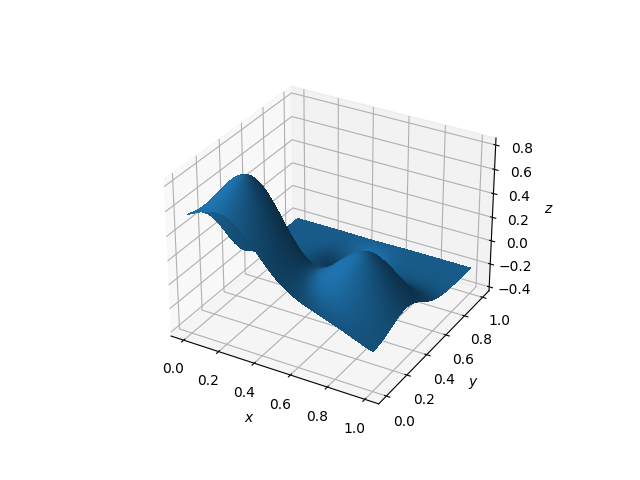
\includegraphics[trim=2.4cm 1cm 1.4cm 1cm, clip,width = 3in]{../assets/actual_franke_plot.png}
  \caption{Shape of Franke's function which will be used as a interpolating goal}
  \label{fig:frankesplot}
\end{figure}


\end{document}